\documentclass{../../text-style}

\texttitle{Введение в Linux}

\begin{document}

\maketitle
\thispagestyle{empty}

\section{Что такое Linux}

Linux --- это семейство Unix-подобных операционных систем, объединённых более-менее общим ядром, набором стандартов и соглашений.
Ядро Linux имеет открытый исходный код, лежит в репозиториях, поддерживаемых сообществом, но имеет зеркало на GitHub (\url{https://github.com/torvalds/linux} (дата обращения: 24.02.2024)).
Вообще, Linux строится вокруг идеи свободного программного обеспечения (хотя Linux, Free Software Foundation и GNU --- это разные вещи, их не надо путать), поэтому сообщество очень щепетильно относится к защите от vendor lock-in, поэтому на GitHub и подобные хостинги целиком никогда не переедет.

Linux имеет огромное сообщество разработчиков, управляемых по иерархической структуре, в корне которой находится Линус Торвальдс --- собственно, первый разработчик ядра, который начинал писать Linux как студенческую работу на основе идей учебной ОС Minix от Эндрю Танненбаума (который сам по себе очень известный товарищ).
Открытость и вовлечённость кучи людей в процесс имеет свои плюсы и свои минусы:

\begin{itemize}
    \item всё, о чём вы можете подумать, скорее всего, кто-то уже сделал;
    \item пользователи имеют доступ к исходному коду, замечают проблемы, предлагают правки, поэтому популярное ПО (тем более --- ядро), скорее всего, очень стабильно и \enquote{вылизано} до блеска;
    \item никто никому ничего не должен, поэтому не очень популярное ПО может быть откровенно плохим;
    \begin{itemize}
        \item более того, часто разрабатывается красноглазыми школьниками, которые без идей, как программировать, но попасть в какой-нибудь дистрибутив Linux для них мечта --- в ядро их код не берут, но прикладные программы вполне.
    \end{itemize}
    \item нет единых стандартов, архитектуры, процесса, не только для прикладного ПО, но и для важных частей ОС.
\end{itemize}

Применяется Linux сейчас в основном как серверная ОС, и в этом плане она с большим отрывом лидирует (разве что другие UNIX-подобные системы типа FreeBSD, которые неопытный пользователь никогда не отличит от Linux, могут составить ей конкуренцию).
Также Linux, в силу открытости и модульности, применяется для встроенных устройств и разного специализированного оборудования, где нет требований реального времени%
\footnote{Системы жёсткого реального времени должны давать гарантию, что такая-то процедура будет выполнена за такое-то физическое время, например, за 20 миллисекунд. Linux не может давать такой гарантии.}.
Linux также несколько удобнее для профессиональной разработки, особенно для низкоуровневого программирования, под него более зрелый и удобный инструментарий.
Однако и Enterprise-, и веб-, облачная и т.п. разработка тоже часто ведётся на Linux, отчасти потому, что это достаточно удобно, отчасти чтобы быть ближе к окружению, в котором разработанная система будет работать.

Почему не весь мир работает на Linux --- у Linux не очень хороши дела для поддержки конечных пользователей.
Современные дистрибутивы очень дружелюбны (в былые времена иногда приходилось программировать на Си для повседневного пользования компьютером, что не очень), но гораздо хуже обстоят дела с поддержкой аппаратного обеспечения и с играми.
С аппаратным обеспечением дела обычно поправимы --- если производитель не выпускает официально ПО для Linux, это делают энтузиасты, и если что-то не заработало сразу, можно некоторое время пострадать (возможно, попрограммировав на Си), и заработает (в отличие от Windows, где, как правило, если что-то не работает, то всё).
Из того, с чем наверняка придётся столкнуться --- некоторая ненадёжность автоматической настройки дисплеев, так что заставить линуксовый ноутбук правильно выводить на проектор может быть неким вызовом (программировать не придётся, но копаться в конфигах в трёх разных местах --- возможно).
Заставить работать три монитора с разным разрешением от двух видеокарт разных вендоров так, чтобы выполнялось адекватное масштабирование пользовательского интерфейса --- автору так и не удалось.

С играми похуже, сообщество не считает их чем-то полезным, и там часто используются специфичные для Windows технологии, такие как DirectX.
Однако в последнее время игровые движки делаются кроссплатформенными, так что игры на них под Linux в целом работают, хотя иногда странно.
Но есть довольно много игр, которые не работают, и, видимо, никогда не будут.

Linux распространяется в виде дистрибутивов.
Само ядро не имеет никакого пользовательского интерфейса, даже консольного, и его можно понимать как скомпилированную библиотеку, которая всем управляет и предоставляет программный интерфейс для прикладных программ и системных утилит.
Ядро модульное, есть штуки, которые так и называются --- \enquote{модули}, их можно воспринимать как динамически загружаемые библиотеки, которые можно подгружать и выгружать прямо в процессе работы системы, и они обычно нужны для поддержки того или иного оборудования.
Однако чтобы пользователю работать с системой, нужна куча прикладных программ --- во-первых, шелл (shell), интерфейс командной строки, во-вторых, утилиты типа копирования файлов, в-третьих, графическая оболочка, в-четвёртых, пакетный менеджер, отвечающий за установку, обновление и удаление прикладных программ.
Всё это вместе, плюс начальная конфигурация системы, плюс политика обновления ПО и т.п. --- это и есть дистрибутив, то есть готовая к использованию система, которую можно поставить к себе на компьютер и начать ей пользоваться.
Дистрибутивов сотни, даже известных и широкораспространённых десятки.
Есть три-четыре популярных российских, которые на волне импортозамещения и ухода Microsoft стремительно занимают освободившуюся нишу в корпоративной и государственной сферах, и заодно и у обычных пользователей, хотя им приходится отчаянно конкурировать с западными.
Для корпоративных нужд требуется техподдержка, что с западными дистрибутивами может быть трудно, для домашнего использования техподдержка не нужна, поэтому вполне разумный выбор (хотя ходят слухи, что некоторые программы могут потихоньку гадить пользователям из России).

\subsection{Чем Linux хорош для программистов}

Linux популярен в программистском сообществе по целому ряду причин.
Наверное, основная --- бесплатность.
Linux можно ставить на виртуальные машины в каких угодно количествах, не платя за лицензию, а поскольку сейчас повсеместно используется виртуализация и контейнеризация, это может быть критично.
В правильно настроенном сервере \emph{каждый} делающий полезную работу процесс работает в собственном контейнере (или на целой виртуальной машине), так что на лицензиях на Windows и ПО для него даже крупная компания могла легко разориться.
Однако, как обычно, есть нюанс --- бывают и даже вполне распространены платные дистрибутивы.
Бесплатность открытого ПО вовсе не значит, что на нём нельзя зарабатывать --- покупая платный дистрибутив, пользователь покупает отсутствие проблем и техподдержку, если проблемы всё-таки возникнут, плюс, иногда, проприетарные специальные программы и сервисы, которых нет в открытом доступе.
Например, Астра Линукс распространяется именно по такой модели --- есть очень устаревшая бесплатная версия и свежая платная для корпоративных клиентов, с \enquote{правильными} гарантиями безопасности, включая гарантию защиты от \enquote{protestware}%
\footnote{\enquote{Protestware} --- программное обеспечение, которое, помимо полезных функций, пытается донести до пользователя позицию автора по какому-либо политическому или социальному вопросу, вплоть до попытки форматирования диска пользователей, которых автор считает в чём-либо виновными. В мире открытых систем огромной сложности весьма опасно (поскольку может быть \enquote{притянуто} зависимостями), и зачастую крайне неэтично. Не делайте так, какими бы благими ни были ваши намерения.}.

Вторая причина --- конфигурируемость.
Есть готовые дистрибутивы, включающие в себя всё, необходимое для работы.
Есть миниатюрные системы, которые, кроме ядра, имеют программ на 4-5 мегабайт (!), что идеально для работы в контейнерах, потому что контейнеризованному приложению ядро не нужно.
Да и всего, вместе с ядром, вполне можно собрать работоспособный дистрибутив размером чуть больше сотни мегабайт, что позитивно для встроенных устройств и специализированных контроллеров.
Есть дистрибутивы, которые можно целиком собрать из исходников под конкретную архитектуру, есть специализированные системы сборки, которые позволяют собрать ядро и нужные модули и положить поверх только нужные программы и конфигурацию.

Третья причина --- это простое человеческое удобство, если привыкнуть.
Наличие пакетного менеджера и централизованного репозитория с программами позволяет не искать ничего в интернетах, устанавливать всё одной командой и обновлять вообще автоматически.
При этом продвинутая система управления зависимостями поставит всё, что нужно, так, чтобы оно не мешало уже установленному программному обеспечению и библиотеки/вспомогательные программы не дублировались для сотни прикладных программ, как это принято в Windows%
\footnote{Тут, опять-таки, есть нюансы --- зависимости хорошо работают внутри дистрибутива, но если нужного ПО нет в дистрибутиве, есть, но старой версии, или просто в пакете ошибка, поставить его на Linux-систему может быть нетривиально. Поэтому Linux сейчас тоже движется к тому, что в Windows/.NET называется \enquote{xcopy deployment} --- всё, что нужно для работы, приложения носят с собой. На Linux-системах с этим может очень помогать контейнеризация.}.
В Linux традиционно удобная и прилично выглядящая консоль, поскольку по историческим причинам пользователи проводят в консоли очень много времени, там всё вылизано до блеска.
Наверное, требуется некоторое время, чтобы привыкнуть и выучить горячие клавиши выбранного вами шелла (да-да, в Linux консоль не встроена в систему, есть штуки три только популярных консольных оболочки).
Зато потом открывать консоль на Windows уже не захочется.

Кроме всего этого, есть целый ряд инструментов, которые не работают на Windows (и тем более Mac OS) вообще.
Например, отладчик памяти Valgrind (в Visual Studio есть аналог, но Valgrind умеет гораздо больше Visual Studio), эмулятор аппаратного обеспечения QEMU (её вроде как можно запустить под Windows, но я бы не стал даже пытаться), эмулятор процессора Gem5 (там возможность запуска не под Linux разработчиками даже не рассматривается) и т.д. и т.п.
Два последних инструмента могут быть критичны для ряда направлений разработки, включая встроенные системы и компиляторы.

\subsection{История Linux}

Как известно, Linux --- это написанная с нуля как студенческая работа ОС (где-то в 1990 году), позаимствовавшая ряд идей из учебной ОС Minix, которая в свою очередь использовала ряд идей, стандартов и соглашений Unix.
Unix пошла ещё от DEC-овских мэйнфреймов, появилась аж в начале 1970-х (когда создание единой ОС для серийных ЭВМ стало насущной необходимостью, до этого ОС писалась под каждую конкретную машину).
От Unix произошла ОС BSD разных сортов (Berkeley Software Distribution, хотя на самом деле BSD --- это более общая штука, чем ОС).
От BSD --- Mac OS (так что Mac OS более Unix, чем Linux).
Кстати, Windows произошла от MS-DOS (хотя, конечно, была полностью переписана с тех времён), а MS-DOS --- это клон системы CP/M 1974-го года, которая вроде как вообще никакого отношения к Unix не имела.

Вот родословная Unix и Unix-подобных операционных систем:

\begin{center}
    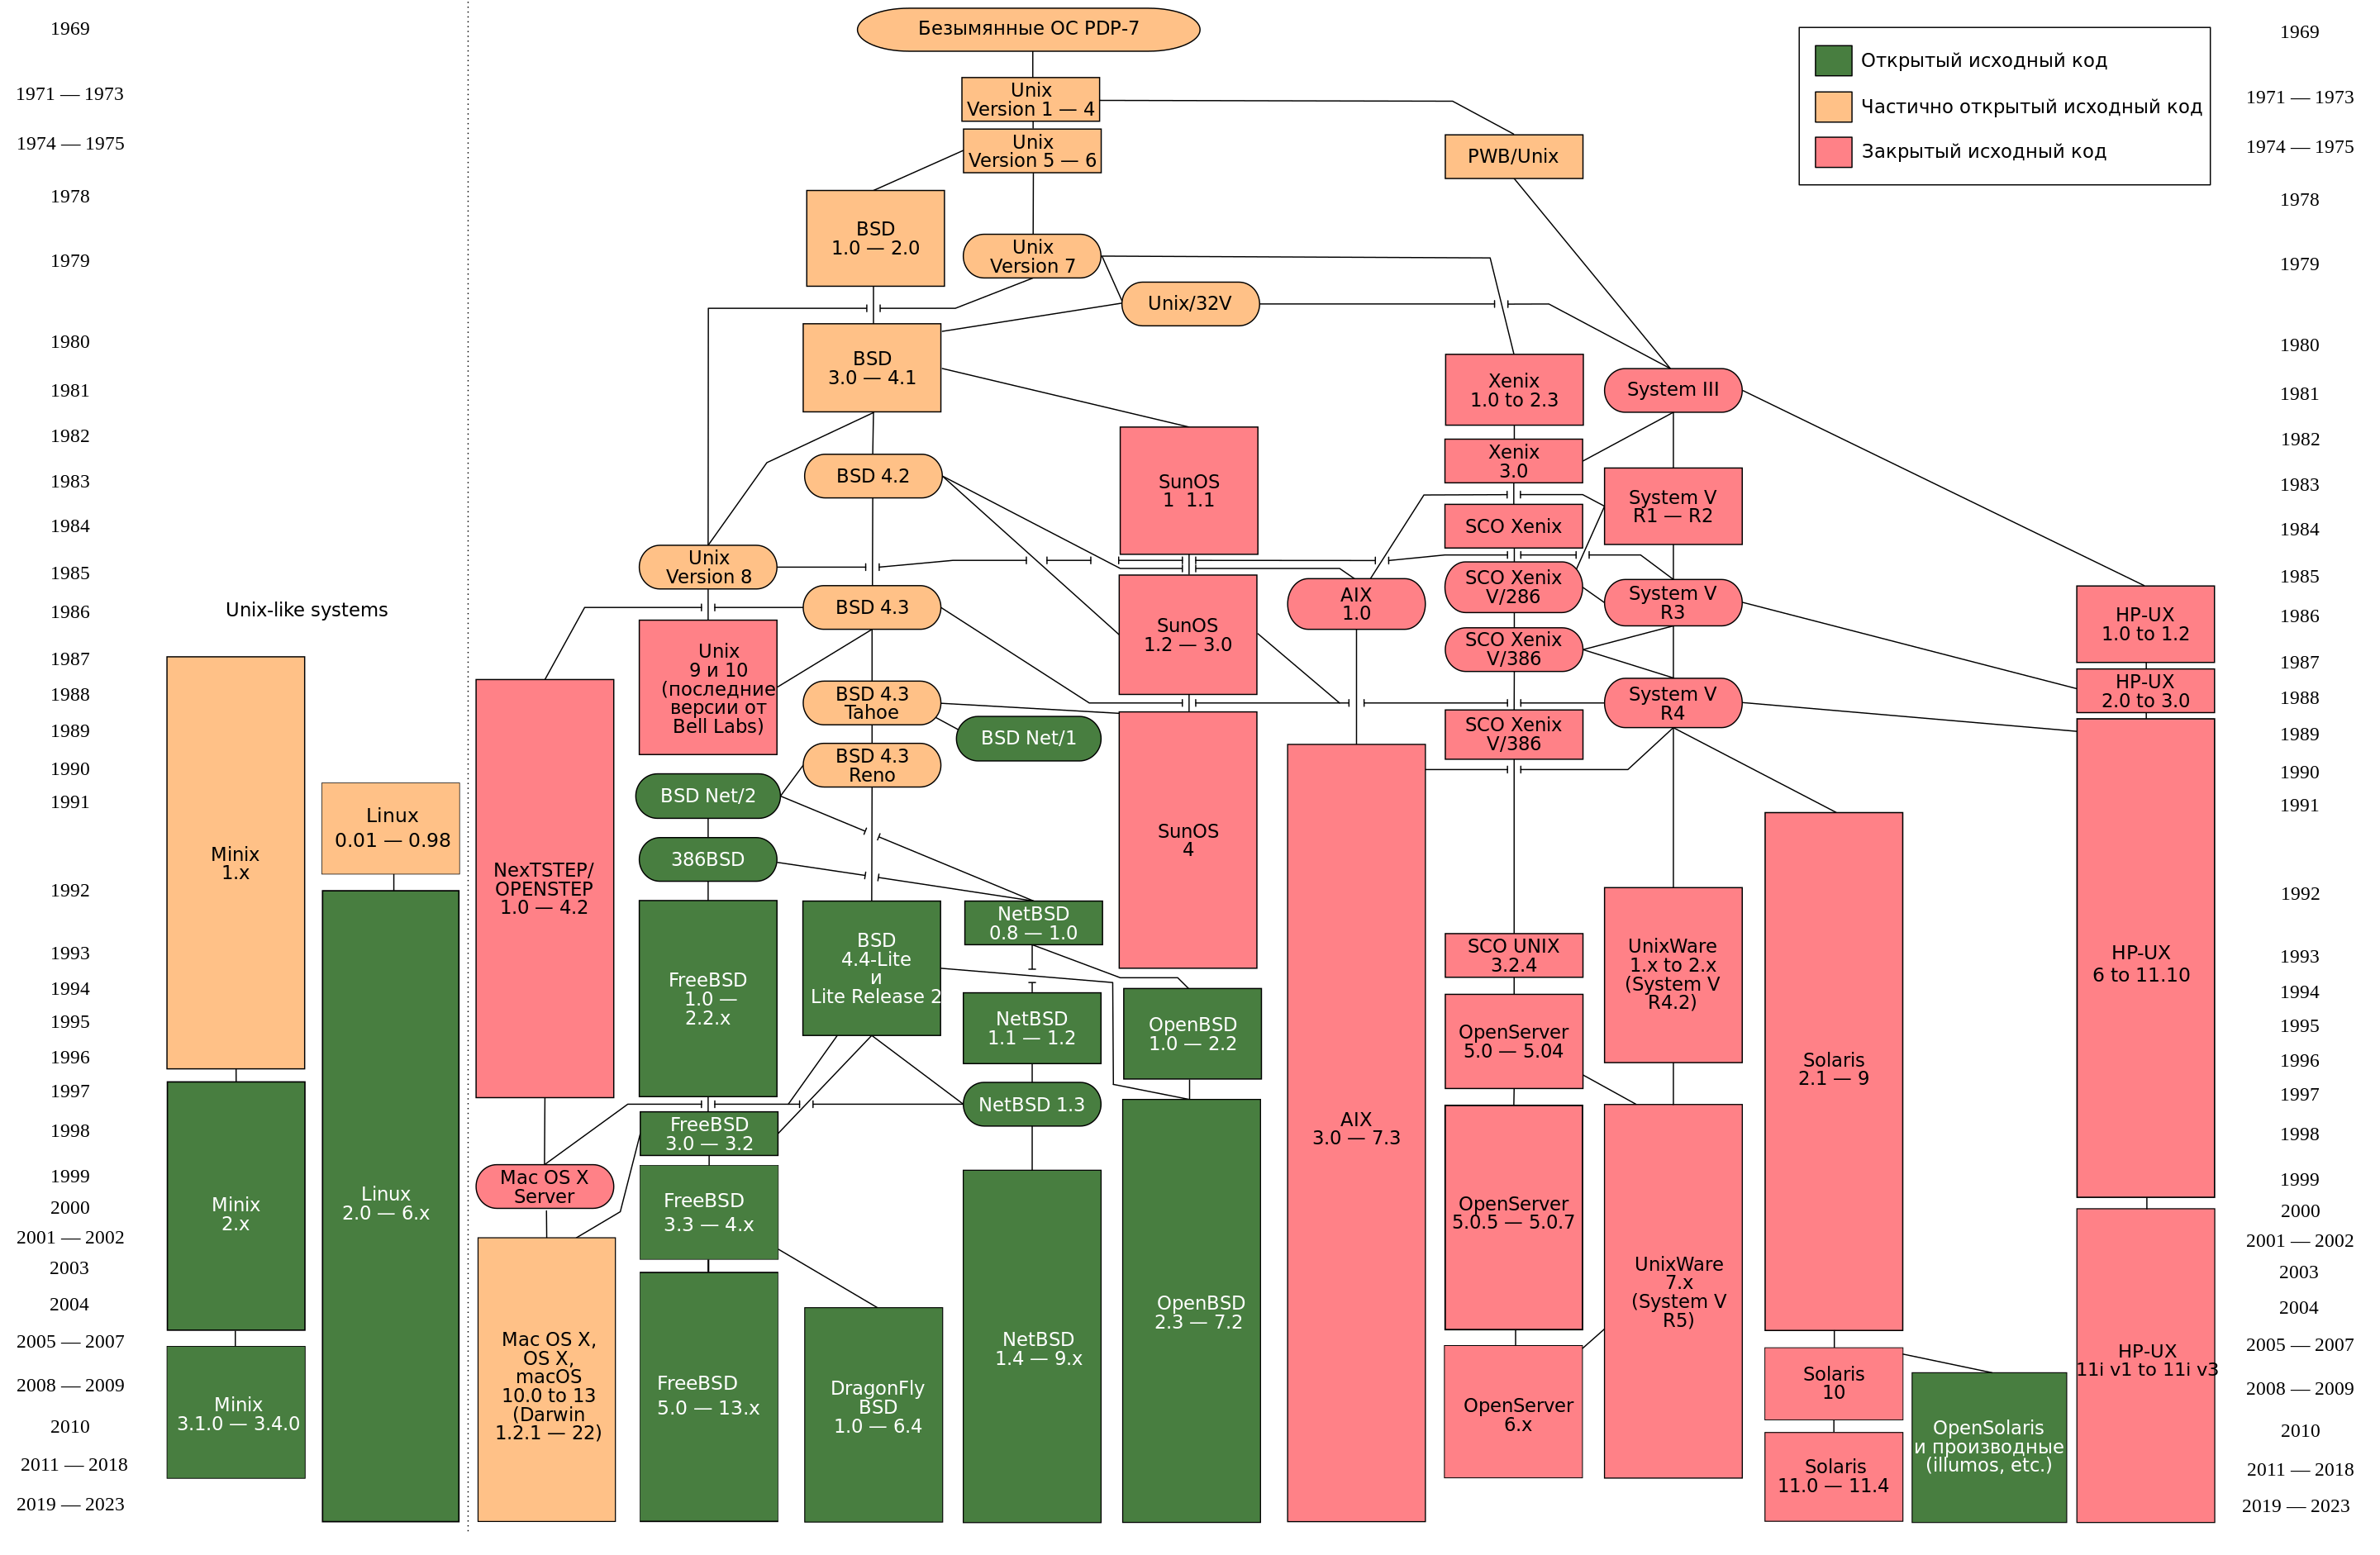
\includegraphics[width=0.9\textwidth]{unixHistory.png}
\end{center}

\subsection{Отличия от Windows}

Тут обсудим отличия Linux от Windows с точки зрения пользователя.
Вообще, это совершенно разные операционные системы, с разной философией, архитектурой и, конечно, пользовательским опытом, однако общего у них тоже довольно много (что неудивительно, похожие задачи всегда влекут похожие решения).
Вот с чем пользователь Windows, который впервые пересаживается на Linux, обязательно столкнётся.

\begin{itemize}
    \item Пакетный менеджер.
        В Linux приложения не скачиваются с непонятных сайтов, как принято в Windows, а ставятся из централизованных репозиториев с помощью установочных пакетов и специальной программы --- того самого пакетного менеджера.
        Причём, если в Windows программы обычно ставятся в Program Files и иногда имеют свою подпапку в папке пользователя, то в Linux приложение оказывается \enquote{размазанным} по файловой системе по определённым правилам, о которых чуть дальше.
        Поэтому установка, удаление, обновление и т.п. делается через пакетный менеджер, просто удалять программу с диска нельзя, и не принято встраивать в программы функциональность автообновления (например, VS Code обновляет себя под Windows, но обновляется силами пакетного менеджера под Linux).
        Пакеты могут зависеть друг от друга, поэтому прикладные программы, как правило, имеют в разы меньшие размеры, чем в Windows --- всё нужное уже, скорее всего, установлено в системе, и если нет, то поставится автоматически и может быть переиспользовано ещё кем-то.
        Пакетная система дистрибуции программного обеспечения уже наверняка знакома --- в Windows есть свой пакетный менеджер Chocolatey (но поскольку он не встроен в систему, о нём мало кто знает), есть Microsoft Store (но там своя атмосфера), ещё есть Android и iOS, где репозиторий централизованный и контролируется производителем.
        В Linux репозиторий обычно привязан к дистрибутиву и один, но никто не мешает добавить сколько угодно дополнительных, и тут это валидная модель распространения программы --- например, VS Code предоставляет репозиторий, где лежат пакеты самого VS Code и зависимостей.
        Скачивать программы с непонятных сайтов тоже можно, тем более что непонятные сайты обычно предлагают удобный способ установки под Linux (например, .NET ставится именно так, скриптом dotnet-install.sh с сайта Майкрософт), но делается это только в случае, если в репозитории дистрибутива нужного пакета нет.
    \item Файловая система различает регистры в именах файлов и папок, так что header.h и Header.h --- совершенно разные файлы.
        Поэтому на всякий случай всё обычно именуется со строчной через подчёркивание или дефис.
        Бывают, конечно, исключения (в дистрибутиве, на котором верстался этот конспект, например, есть директория \enquote{Рабочий стол}).
        У файлов нет атрибута \enquote{скрытый}, поэтому по соглашению скрытые файлы именуются с точки в начале.
        Кстати, все имена файлов --- в UTF-8.
    \item В файловой системе нет понятия \enquote{диск}, дерево файлов и директорий имеет один корень, директорию \enquote{/}.
        Абсолютно всё, включая файлы на разных физических дисках, флешках и сетевых шарах, лежит где-то в поддиректориях \enquote{/}.
        Есть понятие \enquote{монтирование} --- \enquote{прививание} внешней файловой системы внутрь какой-то из директорий \enquote{/}.
        Например, флешка может быть доступна по пути \enquote{/media/user/флешка/}.
        Монтирование можно выполнять вручную, но в подавляющем большинстве случаев оно выполняется само.
    \begin{itemize}
        \item Обратите внимание, слеши в Linux всегда прямые. 
            Windows умеет и так и так. но предпочитает обратные, Linux считает обратный слеш началом escape-последовательности.
    \end{itemize}
    \item Оконный менеджер не является частью операционной системы.
        В Windows управление окошками --- часть функциональности ядра, поэтому поменять их внешний вид и, тем более, функциональность, весьма сложно.
        В Linux есть как отдельные приложения низкоуровневые рисовалки, которые умеют рисовать собственно окна и обрабатывать события пользовательского ввода, так называемые \enquote{окноводы}, которые управляют размерами и размещением окон, и \enquote{среды рабочего стола}, которые добавляют всякие кнопки, панельки, виджеты, эффекты и т.п.
        И это более-менее ортогональные вещи, и по каждому пункту есть выбор, иногда весьма значительный.
        Поскольку всё это весьма конфигурируемо, каждый дистрибутив выглядит по-своему, да ещё и можно настроить под себя практически всё, вплоть до полной смены оконной подсистемы (что не так просто, но возможно).
    \item В Windows можно было набрать что-нибудь вроде \enquote{run.exe}, и если run.exe есть в текущей папке, он запустится.
        Linux скажет, что файл не найден, и начинающие пользователи могут быть шокированы, потому что вот же он лежит.
        Дело в том, что Linux не ищет по умолчанию запускаемые файлы в текущей директории, а сразу идёт смотреть пути из PATH --- по соображениям безопасности, чтобы нельзя было подложить что-то странное в директорию с программой.
        Чтобы запустить что-то из текущей директории, добавьте явную на неё ссылку: \enquote{./run.exe}.
        Ещё у файлов (и директорий) есть атрибут \enquote{исполнимый}, если атрибут не выставлен, запустить программу/скрипт не выйдет даже с точкой.
        Windows понимала, что файл исполнимый, по расширению, Linux тут на расширения не смотрит.
        Выставить атрибут \enquote{исполнимый} можно командой \mintinline{text}{chmod +x имя-файла}.
    \item В Windows большая часть системных настроек была в реестре, который по сути большая иерархическая база данных, которую без regedit.exe даже открыть-то не получится, причём и с regedit.exe там весьма сложно что-то содержательно редактировать и надо либо знать, что делаешь, либо пользоваться программами для настройки.
        В Linux есть правило, что все настройки должны быть человекочитаемыми и человекоредактируемыми.
        Поэтому обычно для конфигурации всего, даже самых дебрей ОС, используются простые текстовые файлы.
        При этом если опций много и файл большой, применяется соглашение с разделением такого конфига на несколько файлов и выкладыванием их в папку <имя конфига>.d, где файлы перенумерованы в порядке их применения.
        Так что конфиги не только человекочитаемы, но ещё и обозримы и понятны (как правило).
    \item Очень важное различие --- папки в Linux называются директориями.
\end{itemize}


\end{document}
